\subsection{3 预训练}\label{pre-training}

\subsection{3.1 预训练数据}\label{pre-training-data}

Kimi K3 在一个经过精心筛选的语料库上进行预训练，该语料库涵盖四大文本领域——网页文本、代码、数学和知识——以及一个大规模视觉语料库。视觉数据涵盖图像描述、图文交错文档、OCR、感知、视频和视觉编码数据。我们的数据流水线建立在为 Kimi K2 {[}58{]} 开发、并在 Kimi K2.5 {[}59{]} 中进一步优化的流水线基础之上。

文本数据 每个领域通过基于规则的启发式方法、基于分类器的质量评分和去重的组合进行过滤，各领域的采样率由在小模型上的消融实验确定。遵循 Kimi K2 {[}58{]} 的重述（rephrasing）方案，我们使用风格和视角多样化的提示、分块自回归生成以及针对源文档的保真度验证，对知识和数学语料进行重述。

视觉数据 视觉语料库遵循 Kimi K2.5 {[}59{]} 的分类体系，将开源数据集与内部过滤、合成和去重流水线相结合。在训练过程中，坐标监督同时以绝对格式和归一化（{[}0,1{]}）格式提供，从而实现精确且对分辨率鲁棒的定位。除了经典的文本标注图像外，我们还大幅扩展了程序化多模态数据，将代码片段与其渲染视觉效果配对，覆盖 SVG、3D 资产、网页、游戏和 CAD 示意图等特定领域格式。

\subsection{3.2 缩放定律}\label{scaling-law}

综合来看，前述各节所描述的架构、数据和训练改进共同定义了我们的新模型系列。由于这些变化也改变了最优训练范式，我们进行了专门的缩放定律研究，以重新调优关键超参数，包括批量大小、学习率、每参数 token 比（TPP）以及模型形状。在留出的 OOD 验证数据上评估，图 7 中的缩放定律曲线显示，这些改进整体上带来了相对于 Kimi K2 约 2.5 倍的缩放效率提升。表 1 提供了 Kimi K2 与 Kimi K3 之间详细的架构对比，突出展示了促成这一提升的结构性变化。

我们的缩放定律研究一致表明余弦衰减优于 Warmup Stable Decay (WSD) {[}46{]}，因此我们采用余弦衰减作为默认学习率调度策略。我们在固定的最低学习率下比较了余弦衰减和 WSD。尽管先前工作报道 WSD 可以匹敌甚至超越余弦衰减，但我们观察到两种调度策略的最优超参数存在显著差异。即使在相同的模型规模和训练 token 预算下，它们的最优峰值学习率和批量大小也大相径庭。因此，使用同一组超参数来比较两种调度策略可能会不公平地偏袒其中一方，仅仅是因为那些超参数与它更匹配。为确保公平比较，我们为每种调度策略分别进行了独立的缩放定律搜索。在各自的最优超参数设置下，余弦衰减始终取得比 WSD 更低的最终损失。

\pandocbounded{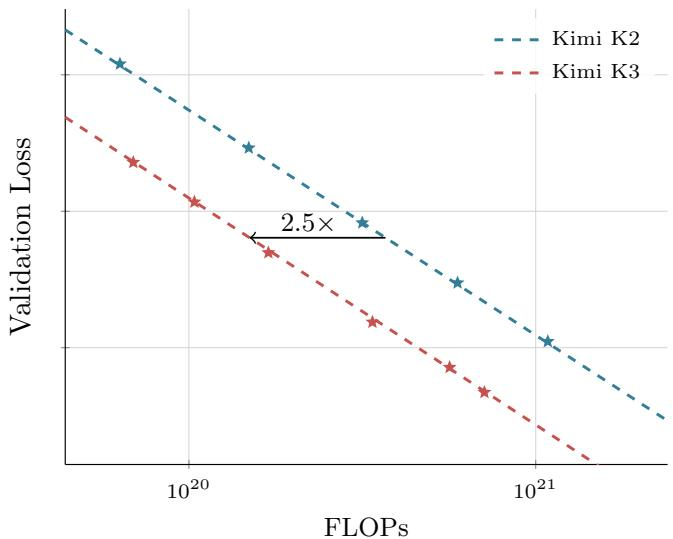
\includegraphics[keepaspectratio,alt={image}]{images/261f163434503a607219080f90e0142b42118835e5f309e187aee887308dc76c.jpg}}

图 7: Kimi K2 和 Kimi K3 的拟合缩放定律曲线。Kimi K3 相比 Kimi K2 实现了 2.5 倍的缩放效率提升。

表 1: Kimi K2 与 Kimi K3 的架构对比。

{\def\LTcaptype{none} % do not increment counter
\begin{longtable}[]{@{}|l|l|l|l|@{}}
\toprule\noalign{}
\endhead
\bottomrule\noalign{}
\endlastfoot
\hline
& Kimi K2 & Kimi K3 & Δ \\
\hline
架构 & MoE & MoE & - \\
\hline
层数 & 61 & 93 & ↑ 52\% \\
\hline
总参数量 & 1.04T & 2.78T & ↑ 167\% \\
\hline
激活参数量 & 32.6B & 104.2B & ↑ 220\% \\
\hline
隐藏维度 & 7,168 & 7,168 & = \\
\hline
潜在 MoE 维度 & - & 3584 (0.5×) & - \\
\hline
每专家 MoE 隐藏维度 & 2,048 & 3,072 & ↑ 50\% \\
\hline
路由专家数 & 384 & 896 & ↑ 133\% \\
\hline
每 token 激活专家数 & 8 & 16 & ↑ 100\% \\
\hline
共享专家数 & 1 & 2 & ↑ 100\% \\
\hline
注意力头数 & 64 & 96 & ↑ 50\% \\
\hline
稠密层数 & 1 & 1 & = \\
\hline
词表大小 & 160K & 160K & = \\
\hline
训练上下文长度 & 128K & 1M & 8× \\
\hline
注意力机制 & MLA & 混合 KDA-MLA & - \\
\hline
激活函数 & SwiGLU & SiTU-GLU & - \\
\hline
注意力层组成 & 61 MLA & 69 KDA + 24 MLA & - \\
\hline
MTP 层数 & 1 层 & 1 层 & = \\
\hline
ViT 总参数量 & - & 401M & - \\
\hline
ViT 层数 & - & 27 层 & - \\
\hline
ViT Patch 大小 & - & 14 & - \\
\hline
ViT 注意力头数 & - & 12 & - \\
\hline
\end{longtable}
}

\subsection{3.3 训练配方}\label{training-recipe}

Kimi K3 采用原生多模态训练策略，语言和视觉从训练伊始就联合优化，而不是通过事后对齐阶段将视觉编码器嫁接到预训练语言模型上。在此范式下，视觉 token 和文本 token 在统一的下一 token 预测目标中交错排列，使共享主干网络能够从一开始就学习统一的多模态表示。

我们使用 Per-Head Muon 优化器（§ 2.5）以及 Kimi K2 中引入的权重裁剪机制来优化模型，同时采用 QB（§ 2.3.3）进行 MoE 负载均衡。我们使用余弦学习率调度，配合 1\% 的线性预热。整个训练过程中权重衰减设为 0.1。

我们的预训练从 8k token 的上下文长度开始，随后在后续训练阶段扩展到 64k token。

\subsection{3.4 长上下文扩展}\label{long-context-extension}

位置编码 Kimi K3 不使用显式位置嵌入（NoPE），而是通过 KDA 的循环门控和衰减机制隐式编码位置信息。因此，模型可以直接外推到 1M token 上下文，而无需任何位置编码修改，例如 RoPE 重缩放或插值 {[}92{]}。

长上下文数据 来自自然来源的长文档和视频包含大量低质量内容，包括近重复项、二进制 blob、截断文件、视频片段和无效的机器生成日志。因此，我们通过一个专门的清洗流水线对其进行处理，该流水线结合了精确去重和模糊去重、针对视频的逐帧感知哈希、基于启发式和分类器的质量过滤以及结构验证。由于真正长且连贯的文档和视频相对于短文本而言十分稀缺，我们对它们进行上采样，以确保在冷却（cooldown）阶段长上下文分布不会被短序列淹没。然而，仅靠长度本身并不能赋予长程能力。为解决这一问题，我们通过精心排列和拼接多模态文档及子任务来合成额外的长上下文数据，使得嵌入其中的任务只有通过关注分散在整个 1M token 上下文中的信息才能解决。这使注意力机制在预期规模上得到训练，防止其退化为局部模式。

渐进式上下文扩展 Kimi K3 支持高达 100 万 token 的上下文窗口。我们通过在训练过程中渐进式扩展上下文窗口来实现这一目标，遵循四阶段课程。窗口在预训练期间从 8K 扩展到 64K token，在冷却阶段从 256K 扩展到 1M token。将昂贵的长序列计算集中在整体训练预算的一小部分内，使得课程既经济高效，又能让模型逐步适应越来越长的依赖关系。使 KDA 层能够进行百万 token 训练的序列维度划分详见 §5.1.2。

